\subsection{Ejercicio 4}
	Como último ejercicio de este trabajo práctico, dado dos archivos binarios de tareas dadas por la materia, fue necesario la implementación del 
\keyword{switcheo} de éstas dos tareas. En pocas palabras, como el procesador no puede realizar varias tareas al mismo tiempo, el sistema intenta simular 
esta condición, otorgándole tiempo, periódicamente, de uso del procesador (\keyword{multitasking}). Se utilizó la interrupción del \keyword{tick} del 
\keyword{clock} para realizar este cambio de tareas.

	Antes de realizarlo, fue necesario concebir un espacio donde poder guardar el contexto de nuestras futuras tareas, así cuando se estén \keyword{switcheando}, 
al volver a tener el control del \code{cpu} en un momento dado, puedan continuar desde donde dejaron su trabajo. El archivo \code{TSS.h} define la 
estructura del espacio donde guardar el contexto. El archivo \code{TSS.c} genera un array de tres de estos espacios (llamados \code{TSS}), el segundo 
para la tarea pintor, y el tercero para la tarea traductor. La primer \code{TSS} se utiliza únicamente para habilitar el \keyword{multitasking}, que en 
breve, pasará a explicarse.

	Estas \code{TSS} ubicadas en memoria, necesitan de descriptores particulares (descriptores de tareas) en nuestra \code{GDT}, para así poder 
ubicarlos. Se generan en el \code{gdt.c} tres descriptores de \code{TSS} entonces, uno para cada una de las recientemente mencionadas. A continuación, 
un gráfico con las componentes del descriptor. 

\begin{center}
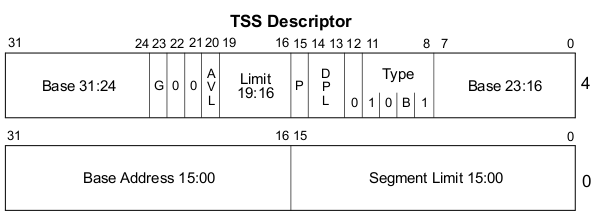
\includegraphics[scale=0.4]{tss_descriptor.png}
\end{center}

Al conocer su tamaño (\code{0x6c} \keyword{bytes}), pudo definirse el límite de los descriptores, tanto como sus atributos. Se dejó para el \code{kernel.asm} 
el trabajo de setear la base.

	Ya ahora en el archivo \code{kernel.asm} nos encargamos de rellenar la información de las \code{TSS} del pintor y del traductor. Guardando sus 
pilas correspondientes (ubicadas en las posiciones dadas por el \keyword{mapeo} de memoria de la materia), los \keyword{flags} de cada uno (0x0202 para 
habilitar interrupciones y cumplir con el \keyword{bit} número 2 prendido requerido por Intel), guardando en cada \code{TSS} el correspondiente directorio 
de páginas de cada uno en el espacio salvaguardado para cada \code{CR3}; guardando todos los registros de propósito general y los registros de segmentación.

	Teniendo las \code{TSS} con la información necesaria para empezar con el \keyword{task switching}, nuestro siguiente paso fue completar los 
descriptores de tares de la \code{GDT} con la base de cada \code{TSS}.

\begin{verbatim}
		mov eax,tsss 
		add eax,TSS_SIZE	;(TSS de pintor, la siguiente es la del traductor) 
		mov word [edi+2],ax		
		shr eax,16 
		mov byte [edi+4],al 
		mov byte [edi+7],ah
\end{verbatim}

La dirección de memoria del comienzo de la TSS se guarda en cada uno de los descriptores. Las siguientes instrucciones se encargan de cargar nuestro 
primer descriptor de \code{TSS} que sólo usamos para iniciar el \keyword{multitasking} y así poder saltar a la primera tarea verdaderamente, que en 
nuestro caso es el pintor. La instrucción \code{ltr} carga el registro pasado por parámetro en el \keyword{task register}, al aplicar entonces el 
\code{jump far} hace un \keyword{switch} del \keyword{task register} a la nueva tarea. Luego la instrucción \code{sti} habilita las interrupciones. 

\begin{verbatim}	
	mov ax,0x20      	
	ltr ax 
	sti 
	jmp 0x28:0 
\end{verbatim}
	
En el archivo \code{isr.asm} fue modificada la interrupción de clock (\code{isr32}), para que además de imprimir en pantalla lo necesario para completar 
el ejercicio 3, también realice el cambio de tareas, es decir, actúe como \keyword{scheduler}. Comparando el \code{CR3} actual de la tarea en curso pudimos 
constatar si lo que se estaba ejecutando era el pintor o el traductor, haciendo un \code{jump far} seleccionando el descriptor de la tarea opuesta a la 
actual, y así generando automáticamente un intercambio de tareas por parte del procesador.

Decidimos utilizar una puerta de interrupción para realizar el \keyword{scheduler} porque, al tener que intercambiar únicamente entre dos tareas, era el
esquema más sencillo de implementar. La rutina comienza comparando el registro \code{CR3} con la dirección \code{0xB000} (directorio de páginas del traductor 
y \keyword{kernel}), para saber qué tarea se está ejecutando actualmente. En el caso de estar en la tarea Pintor la comparación da falsa, y se pasa a 
ejecutar la tarea Traductor mediante un \code{jump far} que carga el 7mo descriptor de la \code{GDT}, que le corresponde a la tarea. Si se está ejecutando el 
Traductor y vuelve a suceder la interrupción entonces la comparación va a resultar verdadera y se realizará el cambio a la tarea Pintor. Algo a tener en cuenta
es que al ejecutarse la rutina de atención de la interrupción, el \code{eip} de la tarea que se estaba ejecutando pasa a apuntar a la rutina de atención. Esto
hace que al saltar a la tarea correspondiente, el \code{eip} que se guarda en la \code{TSS} de la tarea que estaba en ejecución se deja en la instrucción siguiente
al salto. Cuando se vuelve a ejecutar la tarea, lo primero que hace es habilitar las interrupciones (que habían sido deshabilitadas al principio de la rutina) 
y luego ejecuta la instrucción \code{iret} que vuelve el \code{eip} al lugar donde estaba en el momento que fue interrumpida la tarea.


